\documentclass{article}
\usepackage[a4paper, margin=1in]{geometry}
\usepackage{amsmath}
\usepackage{amssymb}
\usepackage{cancel}
\usepackage[dvipsnames, svgnames, x11names]{xcolor}
\usepackage[LGR,T1]{fontenc}
\usepackage[mathletters]{ucs}
\usepackage[utf8x]{inputenc}
\usepackage{enumitem}
\usepackage{graphicx}
\usepackage{nicefrac}
\usepackage{pdfpages}
\usepackage{multicol}
\usepackage{babel}
\usepackage{textgreek}
\usepackage{hyperref}
\usepackage{pifont}
\usepackage{latexsym}
\usepackage{fontawesome}
\usepackage{listings}
\tolerance=1
\hbadness=10000
\emergencystretch=\maxdimen
\hyphenpenalty=10000
\newcommand{\lnb}{\vspace{0.3cm}\\}
\newcommand{\spc}{\vspace{0.3cm}}
\newcommand{\bspc}{\vspace{0.5cm}}
\newcommand{\ans}[1]{\textcolor{DarkSlateGray}{#1}}
\newcommand{\mtr}[2]{\left[{\begin{array}{#1} #2 
	\end{array}}\right]} 
\newcommand{\func}[3]{#1=\left\{{\begin{array}{#2} #3 
	\end{array}}\right.} 
\newcommand{\bcItem}[2]{\item[\textbf{#1}] \textbf{#2}}
\newcommand{\f}[2]{\dfrac{#1}{#2}}
\newcommand{\eval}{\big |}
\newcommand{\Eval}{\bigg |}
\newcommand{\abs}[1]{\bigg| #1 \bigg|}
\newcommand{\restarteq}{\setcounter{equation}{0}}
\newcommand{\nf}[2]{\nicefrac{#1}{#2}}
\newcommand{\cand}{\quad&\wedge\quad}
\newcommand{\cor}{\quad&\vee\quad}
\newcommand{\nand}{\quad\wedge\quad}
\newcommand{\nor}{\quad\vee\quad}
\newcommand{\thus}{\therefore\quad}
\newcommand{\answer}{\textbf{Answer.\quad}}
\newcommand{\If}{\mbox{if }}
\newcommand{\si}{\mbox{si }}
\newcommand{\br}{\vspace{0.2cm}\\}
\newcommand{\remark}{\textcolor{red}{*}}
\newcommand{\p}[1]{\textcolor{DeepPink4}{#1}}
\newcommand{\fig}[2]{\begin{center}
		\includegraphics[scale=#1]{#2}
\end{center}}

\begin{document}
	
	\lstset{basicstyle=\footnotesize\ttfamily,breaklines=true}
	\part*{Informe de Cambios y Funcionalidad}
	\textcolor{gray}{\emph{Melany Monroy Icaza}}
	
	\section*{Introducción}
	
	En el levantamiento del proyecto se encontraron algunos errores que se 
	han corregido satisfactoriamente para que el proyecto sea levantado y 
	funcional. En el presente informe se recogen los errores específicos y 
	las medidas que se tomaron para abordarlos. Se clasifican estos errores 
	por ambientes: backend y frontend, y se adjunta evidencia del 
	funcionamiento tras las correcciones del modo solicitado.
	
	\section*{Backend - Spring Boot}
	
	\subsection*{Field \emph{name} Missing}
	
	La prueba de funcionamiento comenzó levantando el backend. El primer 
	error que se encontró al ejecutar el comando \texttt{./mvnw 
	spring-boot:run} indicaba que faltaba un campo requerido en la 
	\emph{entity}, "name". Para solucionar este error se aumentó el campo 
	"name" en el archivo que se halla en el directorio 
	\emph{/sevuelo-backend/src/main/java/ec/sevolutivo/sevuelos/sevuelos/domain/Request.java}
	 como se ilustra a continuación.
	
	\begin{lstlisting}
@NotNull
@Size(max = 100)
@Column(name = "name", length = 100, nullable = false)
private String name;

...

public String getName() {
	return name;
}

public void setName(String name) {
   this.name = name;
}
	\end{lstlisting}
	
	\subsection*{Database configuration}
	
	Una vez arreglado el error, se pudo notar que en el archivo 
	"aplication.properties" no había contenido alguno y que no había una 
	conexión a una base de datos regular (mySql, Oracle, Postgres). La 
	elección de Postgres como base de datos requería incluir en el archivo 
	"pom.xml" la dependencia necesaria, como figura a continuación.

	\begin{lstlisting}
<dependency>
   <groupId>org.postgresql</groupId>
	<artifactId>postgresql</artifactId>
	<scope>runtime</scope>
</dependency>
	\end{lstlisting}
	
	Siguiendo esta elección, se eliminó la dependencia a "h2" que además 
	generaba conflicto. A continuación, se detallaron las configuraciones 
	adecuadas en aplication.properties, de la siguiente manera.
	
\begin{lstlisting}
server.port=${port:8080}
spring.datasource.url=jdbc:postgresql://localhost:5432/db_prueba
spring.datasource.username=theda
spring.datasource.password=postgretheda
spring.datasource.driver-class-name=org.postgresql.Driver
spring.jpa.properties.hibernate.dialect=org.hibernate.dialect.PostgreSQLDialect

spring.jpa.hibernate.ddl-auto=create
\end{lstlisting}

	nótese que en la línea \texttt{spring.jpa.hibernate.ddl-auto=create} se 
	especifica la opción \texttt{create} para que la base de datos se cree 
	(o sobreescriba) una vez se corra el comando para instalar 
	\texttt{./mvnw clean install}. En caso se quiera únicamente actualizar 
	una base de datos ya existente se debe especificar la opción 
	\texttt{update}. Se ejecutó el comando:

\begin{lstlisting}
./mvnw clean install -DskipTests
\end{lstlisting}

	Para instalar la aplicación y crear la base de datos se ejecutó el 
	comando arriba indicado y se usó la bandera 
	\texttt{DskipTests} para saltar las pruebas unitarias y evitar así 
	conflictos por falta de configuración en estas. \\
	
	Una vez realizado todo esto, el servidor en el puerto 8080 para el 
	backend fue levantado exitosamente.
	
	\section*{Frontend - ReactJS}
	
	\subsection*{Package version}
	
	Se hallaron dos errores en el archivo \texttt{package-lock.json}:
	\begin{enumerate}
		\item El primero se encontraba en la versión de \emph{react} 
		especificado en \texttt{"dependencies"}. La línea original de código 
		se mostraba \texttt{"react": " \^118.2.0",}, lo que se cambió por 
		\texttt{\^18.2.0}.
		\item El segundo error era en la especificación de 
		\texttt{babel-loader} y \texttt{webpack}. Estas especificaciones 
		causaron conflicto porque al ejecutar \texttt{npm install} para 
		instalar la aplicación de react, el módulo 
		\emph{react-scripts} ya cargaba una versión actualizada del webpack 
		y babel-loader.
	\end{enumerate}
	
	Una vez corregidos ambos errores se ejecutó primero \texttt{npm 
	install} seguido de \texttt{npm start}.
	
	\subsection*{Http Request}
	
	La aplicación indicaba una pestaña titulada "New Request" y otra que se 
	mostraba al ingreso (establecida «por defecto») titulada "Request". 
	Estaba claro que el formulario en New Request tenía que ingresar datos 
	en la tabla que se mostraría en Requests. Se realizó la prueba y el 
	primer error que hubo es respecto al CORS. Para solucionar esto, en el 
	backend, en el archivo \emph{RequestResource.java} se añadió la URL que 
	estaba siendo denegada en la annotation @CrossOrigin: 
	\emph{http://localhost:3000/requests}. Se procedió a realizar la prueba 
	nuevamente, obteniendo un error con el status http 500, error interno 
	del servidor. Esto indicaba que había un problema ya sea con el cuerpo 
	de la petición http hacia el server, o con el modo en que el server 
	procesaba tal petición. Para esto se imprimió el http request que se 
	generaba al presionar "save" en "New Request" y se verificó que los 
	datos ingresados en el formulario estaban siendo procesados sin 
	problema desde el frontend. Para verificar el error específico en el 
	server se hizo uso de Postman. Al hacer la petición http a través de 
	Postman se pudo visualizar nuevamente el error de código http 500. 
	Revisando el terminal se pudo observar lo siguiente
	
\begin{lstlisting}
jakarta.validation.ConstraintViolationException: Validation failed for 
classes [ec.sevolutivo.sevuelos.sevuelos.domain.Request] during persist 
time for groups [jakarta.validation.groups.Default, ]
List of constraint violations:[
	ConstraintViolationImpl{interpolatedMessage='must not be null', 
	propertyPath=name, rootBeanClass=class 
	ec.sevolutivo.sevuelos.sevuelos.domain.Request, 
	messageTemplate='{jakarta.validation.constraints.NotNull.message}'}
]
\end{lstlisting}

	Esto indicaba que, por supuesto, al incluir el campo \emph{name} tal 
	como se indica en la sección \emph{Backend} el campo no podría estar 
	nulo. En este punto, se podría haber escogido dos caminos: modificar la 
	entity para que el campo \emph{name} acepte valores nulos, o mandar en 
	el http request el nombre además del pasajero y el destino. Por 
	simpleza se escogió modificar el http request, con la siguiente 
	modificación:
	
\begin{lstlisting}
const onSubmit = (data: any) => {
    const newRequest = defaultValue;
    newRequest.name = data.passenger;
    newRequest.passenger = data.passenger;
    newRequest.destination = data.destination;
    createRequest(newRequest);
    reset();
 };
\end{lstlisting}
	Nótese la línea ingresada \texttt{newRequest.name = data.passenger;} 
	donde se especifica que el nombre va a ser el mismo que el ingresado en 
	el campo \emph{passenger}, y la línea borrada 
	\texttt{window.location.href = "/requests"}. Habiendo hecho las dos 
	primeras pruebas se procedió a verificar si se puede obtener la 
	respuesta de la petición http con estado 200 para que la página 
	"refresque" una vez que el payload ha sido exitosamente procesado y la 
	base de datos cargada. Al ser evidente en la prueba 3 que esto no sería 
	posible en el archivo \emph{new-request.tsx} se procedió a modificar la 
	función importada desde \emph{request.service.ts} 
	\texttt{createRequest} de la siguiente manera.
	
	\begin{lstlisting}
export const createRequest = (request: IRequest) => {
  const requestUrl = `${apiUrl}/requests`;
  return axios.post(requestUrl, request).then((response:any)=>{
    if(response.status==200){
      window.location.href = "/requests"
    }
  });
};
	\end{lstlisting}
	
	Con esto se realizó la prueba número 4 y se pudo verificar que el 
	aplicativo funcione acorde a lo esperado. En la Figura 1 se puede 
	verificar el resultado.
	
	\begin{figure}[!h]
		\centering
		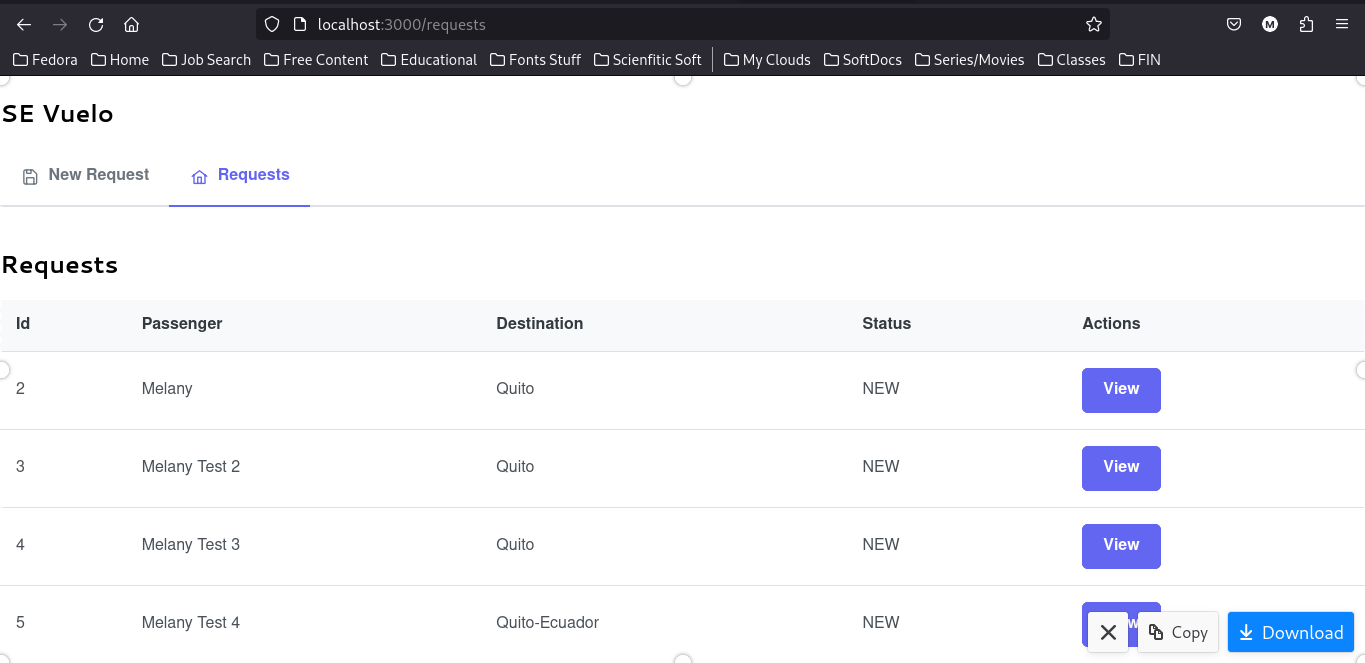
\includegraphics[scale=0.33]{browser.png}
		\caption{Captura de pantalla con los datos siendo ingresados 
		adecuadamente.}
	\end{figure}
	
	En la Figura 2 se puede apreciar que las entradas efectivamente 
	provienen y han sido guardadas exitosamente en la base de datos.
	
	\begin{figure}[!h]
		\centering
		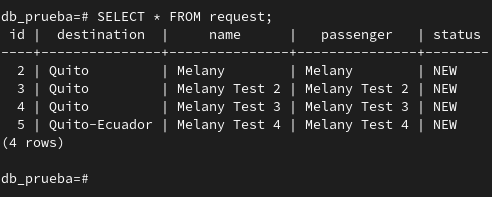
\includegraphics[scale=0.40]{terminal.png}
		\caption{Captura de pantalla con los datos siendo ingresados 
		adecuadamente.}
	\end{figure}
\end{document}